% !TEX root = ../../ctfp-reader.tex

\lettrine[lhang=0.17]{Y}{ou've seen how to model} types and pure functions as a category. I also
mentioned that there is a way to model side effects, or non-pure
functions, in category theory. Let's have a look at one such example:
functions that log or trace their execution. Something that, in an
imperative language, would likely be implemented by mutating some global
state, as in:

\begin{Verbatim}
string logger;

bool negate(bool b) {
    logger += "Not so! ";
    return !b;
}
\end{Verbatim}
You know that this is not a pure function, because its memoized version
would fail to produce a log. This function has \newterm{side effects}.

In modern programming, we try to stay away from global mutable state as
much as possible --- if only because of the complications of
concurrency. And you would never put code like this in a library.

Fortunately for us, it's possible to make this function pure. You just
have to pass the log explicitly, in and out. Let's do that by adding a
string argument, and pairing regular output with a string that contains
the updated log:

\begin{Verbatim}
pair<bool, string> negate(bool b, string logger) {
    return make_pair(!b, logger + "Not so! ");
}
\end{Verbatim}
This function is pure, it has no side effects, it returns the same pair
every time it's called with the same arguments, and it can be memoized
if necessary. However, considering the cumulative nature of the log,
you'd have to memoize all possible histories that can lead to a given
call. There would be a separate memo entry for:

\begin{Verbatim}
negate(true, "It was the best of times. ");
\end{Verbatim}
and

\begin{Verbatim}
negate(true, "It was the worst of times. ");
\end{Verbatim}
and so on.

It's also not a very good interface for a library function. The callers
are free to ignore the string in the return type, so that's not a huge
burden; but they are forced to pass a string as input, which might be
inconvenient.

Is there a way to do the same thing less intrusively? Is there a way to
separate concerns? In this simple example, the main purpose of the
function \code{negate} is to turn one Boolean into another. The
logging is secondary. Granted, the message that is logged is specific to
the function, but the task of aggregating the messages into one
continuous log is a separate concern. We still want the function to
produce a string, but we'd like to unburden it from producing a log. So
here's the compromise solution:

\begin{Verbatim}
pair<bool, string> negate(bool b) {
    return make_pair(!b, "Not so! ");
}
\end{Verbatim}
The idea is that the log will be aggregated \emph{between} function
calls.

To see how this can be done, let's switch to a slightly more realistic
example. We have one function from string to string that turns lower
case characters to upper case:

\begin{Verbatim}
string toUpper(string s) {
    string result;
    int (*toupperp)(int) = &toupper; // toupper is overloaded
    transform(begin(s), end(s), back_inserter(result), toupperp);
    return result;
}
\end{Verbatim}
and another that splits a string into a vector of strings, breaking it
on whitespace boundaries:

\begin{Verbatim}
vector<string> toWords(string s) {
    return words(s);
}
\end{Verbatim}
The actual work is done in the auxiliary function \code{words}:

\begin{Verbatim}
vector<string> words(string s) {
    vector<string> result{""};
    for (auto i = begin(s); i != end(s); ++i)
    {
        if (isspace(*i))
            result.push_back(""); 
        else
            result.back() += *i;
    }
    return result;
}
\end{Verbatim}

\begin{wrapfigure}[11]{R}{0pt}
\raisebox{0pt}[\dimexpr\height-0.75\baselineskip\relax]{
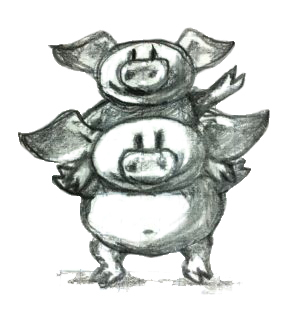
\includegraphics[width=1.83333in]{images/piggyback.jpg}}%
\end{wrapfigure}

\noindent
We want to modify the functions \code{toUpper} and \code{toWords} so
that they piggyback a message string on top of their regular return
values.

We will ``embellish'' the return values of these functions. Let's do it
in a generic way by defining a template \code{Writer} that
encapsulates a pair whose first component is a value of arbitrary type
\code{A} and the second component is a string:

\begin{Verbatim}
template<class A>
using Writer = pair<A, string>;
\end{Verbatim}
Here are the embellished functions:

\begin{Verbatim}
Writer<string> toUpper(string s) {
    string result;
    int (*toupperp)(int) = &toupper;
    transform(begin(s), end(s), back_inserter(result), toupperp);
    return make_pair(result, "toUpper "); 
}

Writer<vector<string>> toWords(string s) { 
    return make_pair(words(s), "toWords ");
}
\end{Verbatim}
We want to compose these two functions into another embellished function
that uppercases a string and splits it into words, all the while
producing a log of those actions. Here's how we may do it:

\begin{Verbatim}
Writer<vector<string>> process(string s) {
    auto p1 = toUpper(s);
    auto p2 = toWords(p1.first);
    return make_pair(p2.first, p1.second + p2.second);
}
\end{Verbatim}
We have accomplished our goal: The aggregation of the log is no longer
the concern of the individual functions. They produce their own
messages, which are then, externally, concatenated into a larger log.

Now imagine a whole program written in this style. It's a nightmare of
repetitive, error-prone code. But we are programmers. We know how to
deal with repetitive code: we abstract it! This is, however, not your
run of the mill abstraction --- we have to abstract \newterm{function
composition} itself. But composition is the essence of category theory,
so before we write more code, let's analyze the problem from the
categorical point of view.

\section{The Writer Category}

The idea of embellishing the return types of a bunch of functions in
order to piggyback some additional functionality turns out to be very
fruitful. We'll see many more examples of it. The starting point is our
regular category of types and functions. We'll leave the types as
objects, but redefine our morphisms to be the embellished functions.

For instance, suppose that we want to embellish the function
\code{isEven} that goes from \code{int} to \code{bool}. We turn it
into a morphism that is represented by an embellished function. The
important point is that this morphism is still considered an arrow
between the objects \code{int} and \code{bool}, even though the
embellished function returns a pair:

\begin{Verbatim}
pair<bool, string> isEven(int n) {
    return make_pair(n % 2 == 0, "isEven ");
}
\end{Verbatim}
By the laws of a category, we should be able to compose this morphism
with another morphism that goes from the object \code{bool} to
whatever. In particular, we should be able to compose it with our
earlier \code{negate}:

\begin{Verbatim}
pair<bool, string> negate(bool b) {
    return make_pair(!b, "Not so! ");
}
\end{Verbatim}
Obviously, we cannot compose these two morphisms the same way we compose
regular functions, because of the input/output mismatch. Their
composition should look more like this:

\begin{Verbatim}
pair<bool, string> isOdd(int n) {
    pair<bool, string> p1 = isEven(n);
    pair<bool, string> p2 = negate(p1.first);
    return make_pair(p2.first, p1.second + p2.second);
}
\end{Verbatim}
So here's the recipe for the composition of two morphisms in this new
category we are constructing:

\begin{enumerate}
\tightlist
\item
  Execute the embellished function corresponding to the first morphism
\item
  Extract the first component of the result pair and pass it to the
  embellished function corresponding to the second morphism
\item
  Concatenate the second component (the string) of the first result
  and the second component (the string) of the second result
\item
  Return a new pair combining the first component of the final result
  with the concatenated string.
\end{enumerate}

If we want to abstract this composition as a higher order function in
C++, we have to use a template parameterized by three types
corresponding to three objects in our category. It should take two
embellished functions that are composable according to our rules, and
return a third embellished function:

\begin{Verbatim}
template<class A, class B, class C>
function<Writer<C>(A)> compose(function<Writer<B>(A)> m1,
                               function<Writer<C>(B)> m2)
{
    return [m1, m2](A x) {
        auto p1 = m1(x);
        auto p2 = m2(p1.first);
        return make_pair(p2.first, p1.second + p2.second); 
    };
}
\end{Verbatim}
Now we can go back to our earlier example and implement the composition
of \code{toUpper} and \code{toWords} using this new template:

\begin{minted}[breaklines,fontsize=\small]{text}
Writer<vector<string>> process(string s) { 
    return compose<string, string, vector<string>>(toUpper, toWords)(s);
}
\end{minted}
There is still a lot of noise with the passing of types to the
\code{compose} template. This can be avoided as long as you have a
C++14-compliant compiler that supports generalized lambda functions with
return type deduction (credit for this code goes to Eric Niebler):

\begin{Verbatim}
auto const compose = [](auto m1, auto m2) { 
    return [m1, m2](auto x) { 
        auto p1 = m1(x);
        auto p2 = m2(p1.first);
        return make_pair(p2.first, p1.second + p2.second);
    };
};
\end{Verbatim}
In this new definition, the implementation of \code{process}
simplifies to:

\begin{Verbatim}
Writer<vector<string>> process(string s) {
    return compose(toUpper, toWords)(s);
}
\end{Verbatim}
But we are not finished yet. We have defined composition in our new
category, but what are the identity morphisms? These are not our regular
identity functions! They have to be morphisms from type A back to type
A, which means they are embellished functions of the form:

\begin{Verbatim}
Writer<A> identity(A);
\end{Verbatim}
They have to behave like units with respect to composition. If you look
at our definition of composition, you'll see that an identity morphism
should pass its argument without change, and only contribute an empty
string to the log:

\begin{Verbatim}
template<class A> Writer<A> identity(A x) {
    return make_pair(x, "");
}
\end{Verbatim}
You can easily convince yourself that the category we have just defined
is indeed a legitimate category. In particular, our composition is
trivially associative. If you follow what's happening with the first
component of each pair, it's just a regular function composition, which
is associative. The second components are being concatenated, and
concatenation is also associative.

An astute reader may notice that it would be easy to generalize this
construction to any monoid, not just the string monoid. We would use
\code{mappend} inside \code{compose} and \code{mempty} inside
\code{identity} (in place of \code{+} and \code{""}). There really
is no reason to limit ourselves to logging just strings. A good library
writer should be able to identify the bare minimum of constraints that
make the library work --- here the logging library's only requirement is
that the log have monoidal properties.

\section{Writer in Haskell}

The same thing in Haskell is a little more terse, and we also get a lot
more help from the compiler. Let's start by defining the \code{Writer}
type:

\src{code/haskell/snippet01.hs}
Here I'm just defining a type alias, an equivalent of a \code{typedef}
(or \code{using}) in C++. The type \code{Writer} is parameterized by
a type variable \code{a} and is equivalent to a pair of \code{a} and
\code{String}. The syntax for pairs is minimal: just two items in
parentheses, separated by a comma.

Our morphisms are functions from an arbitrary type to some
\code{Writer} type:

\src{code/haskell/snippet02.hs}
We'll declare the composition as a funny infix operator, sometimes
called the ``fish'':

\src{code/haskell/snippet03.hs}
It's a function of two arguments, each being a function on its own, and
returning a function. The first argument is of the type
\code{(a -> Writer b)}, the second is
\code{(b -> Writer c)}, and the result is
\code{(a -> Writer c)}.

Here's the definition of this infix operator --- the two arguments
\code{m1} and \code{m2} appearing on either side of the fishy
symbol:

\src{code/haskell/snippet04.hs}
The result is a lambda function of one argument \code{x}. The lambda
is written as a backslash --- think of it as the Greek letter λ with an
amputated leg.

The \code{let} expression lets you declare auxiliary variables. Here
the result of the call to \code{m1} is pattern matched to a pair of
variables \code{(y, s1)}; and the result of the call to \code{m2},
with the argument \code{y} from the first pattern, is matched to
\code{(z, s2)}.

It is common in Haskell to pattern match pairs, rather than use
accessors, as we did in C++. Other than that there is a pretty
straightforward correspondence between the two implementations.

The overall value of the \code{let} expression is specified in its
\code{in} clause: here it's a pair whose first component is \code{z}
and the second component is the concatenation of two strings,
\code{s1++s2}.

I will also define the identity morphism for our category, but for
reasons that will become clear much later, I will call it
\code{return}.

\src{code/haskell/snippet05.hs}
For completeness, let's have the Haskell versions of the embellished
functions \code{upCase} and \code{toWords}:

\src{code/haskell/snippet06.hs}

\src{code/haskell/snippet07.hs}
The function \code{map} corresponds to the C++ \code{transform}. It
applies the character function \code{toUpper} to the string
\code{s}. The auxiliary function \code{words} is defined in the
standard Prelude library.

Finally, the composition of the two functions is accomplished with the
help of the fish operator:

\src{code/haskell/snippet08.hs}

\section{Kleisli Categories}

You might have guessed that I haven't invented this category on the
spot. It's an example of the so called Kleisli category --- a category
based on a monad. We are not ready to discuss monads yet, but I wanted
to give you a taste of what they can do. For our limited purposes, a
Kleisli category has, as objects, the types of the underlying
programming language. Morphisms from type $A$ to type $B$ are functions that
go from $A$ to a type derived from $B$ using the particular embellishment.
Each Kleisli category defines its own way of composing such morphisms,
as well as the identity morphisms with respect to that composition.
(Later we'll see that the imprecise term ``embellishment'' corresponds
to the notion of an endofunctor in a category.)

The particular monad that I used as the basis of the category in this
post is called the \newterm{writer monad} and it's used for logging or
tracing the execution of functions. It's also an example of a more
general mechanism for embedding effects in pure computations. You've
seen previously that we could model programming-language types and
functions in the category of sets (disregarding bottoms, as usual). Here
we have extended this model to a slightly different category, a category
where morphisms are represented by embellished functions, and their
composition does more than just pass the output of one function to the
input of another. We have one more degree of freedom to play with: the
composition itself. It turns out that this is exactly the degree of
freedom which makes it possible to give simple denotational semantics to
programs that in imperative languages are traditionally implemented
using side effects.

\section{Challenge}

A function that is not defined for all possible values of its argument
is called a partial function. It's not really a function in the
mathematical sense, so it doesn't fit the standard categorical mold. It
can, however, be represented by a function that returns an embellished
type \code{optional}:

\begin{Verbatim}
template<class A> class optional {
    bool _isValid;
    A _value;
public: 
    optional()    : _isValid(false) {}
    optional(A v) : _isValid(true), _value(v) {}
    bool isValid() const { return _isValid; }
    A value() const { return _value; }
};
\end{Verbatim}
As an example, here's the implementation of the embellished function
\code{safe\_root}:

\begin{Verbatim}
optional<double> safe_root(double x) {
    if (x >= 0) return optional<double>{sqrt(x)}; 
    else return optional<double>{};
}
\end{Verbatim}
Here's the challenge:

\begin{enumerate}
\tightlist
\item
  Construct the Kleisli category for partial functions (define
  composition and identity).
\item
  Implement the embellished function \code{safe\_reciprocal} that
  returns a valid reciprocal of its argument, if it's different from
  zero.
\item
  Compose \code{safe\_root} and \code{safe\_reciprocal} to implement\\
  \code{safe\_root\_reciprocal} that calculates \code{sqrt(1/x)}
  whenever possible.
\end{enumerate}